\chapter{面向基于深度学习侧信道分析的通用数据增强方法}\label{chap:search1}{
	
	%深度学习技术在侧信道攻击领域中得到了诸多应用,但样本数量不足的情况在实际中经常出现,这严重制约深度神经网络训练效果,甚至会直接影响攻击性能。因此,探讨样本数量有限情况下的数据增强方法,并讨论其对提升基于深度学习的侧信道攻击效果的实际影响,具有重要的现实意义。
	在深度学习的训练阶段对训练数据集进行数据增强可以使训练出的模型更准确,进而降低DL-SCA\chenggongtiaoshu 。然而,当前已有数据增强方法的参数选取通常高度依赖专家知识,且只适合对特定算法实现数据集进行数据增强。因此,构造一个适用于多种算法实现数据集的通用数据增强方法、自适应地选取数据增强参数,具有重要现实意义。
	
	本文选取了不同的AES实现作为分析目标,从数据增强的角度出发,研究减小成功实施DL-SCA所使用的能量迹条数的具有通用性的方法。分析目标包括无防护AES硬件实现、无防护AES软件实现、掩码(和随机延迟)防护AES软件实现以及随机延迟防护AES软件实现,这些实现对应的数据集分别为AES\_HD、DPA v4、ASCADf(N=0/N=50/N=100)、AES\_RD,他们都是侧信道领域权威公开数据集。本文提出了一种通用数据增强方法,其核心思想是采用模拟退火机制依据反馈信号自适应地选择数据增强策略参数。该方法主要由三个核心组件构成:采用模拟退火机制的主控制器、采用组合式数据增强机制的数据增强单元以及提供侧信道攻击代价反馈信号的攻击评估单元。以无防护软件和硬件AES实现、随机延迟和掩码防护AES软件实现为分析目标,在相应的本领域公开数据集上,开展了深度学习侧信道攻击实验对比研究,验证了本文所提出通用数据增强方法的有效性。具体地,在AES\_HD、DPA v4、ASCADf(N=0/N=50/N=100)三种数据集五个场景下,与未采用数据增强方法的DL-SCA效果相比,\chenggongtiaoshu 分别降低21\%、25\%、24\%、48\%以及5\%。在AES\_HD、DPA v4、ASCADf(N=0/N=50)三种数据集四个场景中,与采用其他数据增强方法的DL-SCA效果相比,\chenggongtiaoshu 分别降低22\%、40\%、10\%以及30\%。
	
	{\color{\xchange}
	
	\secref{sec:framework}对通用数据增强方法进行概念上的介绍,\secref{sec:intoreal}详细说明在AES实现上进行实验时通用数据增强方法这一概念的实例化结果,\secref{sec:realexp}汇报了采用通用数据增强方法DL-SCA技术效果。
	}
	
	\section{通用数据增强方法框架}\label{sec:framework}
	应用通用数据增强方法的侧信道分析框架如\figureref{fig:myframe}所示。该框架用于搜索最佳数据增强策略参数,其设计受到AutoAugment\citep{Cubuk19}的启发,它包含自适应数据增强方法、深度学习模型(见\subsref{subs:conceptdlsca})以及对应数据集三部分。其中,本研究提出的通用数据增强方法包含三个核心组件:主控制器(见\subsref{subs:conceptcontroller})、数据增强单元(见\subsref{subs:conceptcda})以及攻击评估单元(见\subsref{subs:concepteva}),其核心思想是采用模拟退火机制依据反馈信号自适应地调整数据增强策略参数。
	
	\begin{figure}[!h]
		\centering
		\begin{tikzpicture}[node distance=45pt, auto]
		% 定义节点样式
			\tikzstyle{reg} = [rectangle, draw,text centered]
			\tikzstyle{block} = [draw, rounded corners,align=center]
			\tikzstyle{data} = [draw, trapezium, trapezium left angle=70, trapezium right angle=110,align=center]
			%\tikzstyle{arrow} = [thick,->,>=stealth]
			
			%绘制节点
			\node [block,minimum width=200pt] (controller) {主控制器};
			\node [block,below of=controller, xshift=70pt](cda){数据增强单元};
			\node [block,below of=controller, xshift=-70pt](eva){攻击评估单元};
			\node [block,below=90pt of controller,minimum width=150pt](dlsca){深度学习模型};
			\node [data,below of=dlsca] (dataset){数据集};
			
			\draw [dashed] ([xshift=-25pt,yshift=10pt]controller.north west) rectangle ([xshift=25pt,yshift=-69pt]controller.north east) node [midway, yshift=5mm, above] {};
			\node at ([xshift=0,yshift=30pt]controller.north west)[anchor=north west]{通用数据增强方法};
			%		\path let \p1=(dataset.south west), \p2=(dataset.north west), \p3=(dataset.north east), \p4=(dataset.south east) in
			%		coordinate (A) at (\p1) 
			%		coordinate (B) at (\p2)
			%		coordinate (C) at (\p3)
			%		coordinate (D) at (\p4);
			
			
			\coordinate (controllersouth) at ($(controller.south)$);
			\coordinate (evanorth) at ($(eva.north)$);
			\coordinate (cdanorth) at ($(cda.north)$);
			\coordinate (evaend) at ($(eva.south)+(-20pt,0)$);
			\coordinate (evaend2) at ($(eva.south)+(+5pt,0)$);
			\coordinate (cdaend) at ($(cda.south)+(+20pt,0)$);
			\coordinate (cdastart) at ($(cda.south)+(-5pt,0)$);
			\coordinate (dlscanorth) at ($(dlsca.north)$);
			
			
			\draw[->] (dataset) -|node[pos=0.4,below] {算法输入、输出} (evaend);
			\draw[->] (dataset) -|node[pos=0.3,above] {验证标签} (evaend);
			\draw[->] (dataset) -|node[pos=0.3,below] {训练数据} (cdaend);
			\draw[->] (dataset) -|node[pos=0.3,above] {训练标签} (cdaend);
			
			\draw[->] (cdastart) --node[pos=0.3,left] {数据增强后} (cdastart|-dlscanorth);
			\draw[->] (cdastart) --node[pos=0.7,left] {的训练集} (cdastart|-dlscanorth);
			\draw[->] (evaend2|-dlscanorth) --node[pos=0.7,right] {验证数据} (evaend2);
			\draw[->] (evaend2|-dlscanorth) --node[pos=0.3,right] {预测结果} (evaend2);
			\graph{
				(evanorth)->["攻击代价"](evanorth|-controllersouth);
				(cdanorth|-controllersouth)->["数据增强策略参数" left](cdanorth);
				(dataset)->["验证数据"](dlsca);
				%(cdastart)->(cdastart|-dlscanorth);
				%(evaend2|-dlscanorth)->(evaend2);
			};
		\end{tikzpicture}
		\bicaption{\enspace 基于通用数据增强方法的侧信道分析框架概览}{\enspace Overview of the framework based on the general data augmentation method}
		\label{fig:myframe}
	\end{figure}
	{\color{\dupc}
			
	通过\figureref{fig:myframe}所示的攻击框架,我们将侧信道领域寻找最佳数据增强策略的问题转化为一个搜索问题。\figureref{fig:myframe}中各个部分与搜索问题的映射关系具体如下。
	
	首先,主控制器扮演着搜索问题中方案决策者角色,负责提供优化方向和指导。它依据反馈的攻击代价信号来不断调整并更新数据增强策略参数,提高侧信道分析技术效果。
	
	其次,数据增强单元充当着搜索问题中命令解析者角色,负责解析和实施主控制器给出的数据增强策略。它依据数据增强策略参数,对原始训练集进行数据增强,并输出数据增强后的训练集。
	
	随后,深度学习模型对应于搜索问题中的任务执行者角色,利用数据增强单元处理后的训练集进行训练,并通过验证集对正确密钥进行预测,得出正确密钥的预测结果和真实结果。它是整个框架中负责执行具体攻击任务和评估攻击效果的部分。
	
	最后,攻击评估单元对应于搜索问题中的评估者角色,用于计算攻击代价并反馈给主控制器。它利用攻击代价的计算公式,结合深度学习模型的预测结果和真实结果,将侧信道分析结果转化为主控制器所需要的攻击代价反馈信号。
	}
	\subsection{主控制器}\label{subs:conceptcontroller}
	如果将数据增强策略参数视为深度学习模型的某种超参数,那么主控制器的功能就是根据反馈信号自动地筛选超参数,以取代需要依赖大量专家知识的人工选择方法。
	
	{\color{\dupc}
		
		我们使用模拟退火机制构建主控制器。模拟退火是一种高效的启发式搜索算法,它具有良好的全局搜索能力。我们从多种自适应数据增强方法中选择模拟退火机制作为主控制器的原因如下。 
		
		首先,在自适应数据增强方法中,搜索算法的反馈信号灵活性高,可以自定义。自适应数据增强是指使用强化学习、元学习或搜索算法,自动地寻找最优数据增强策略的一类方法。搜索算法可以使用任何自定义的反馈信号,可以将适用于侧信道分析的攻击代价作为反馈信号。而其他的自适应数据增强方法如强化学习、元学习等则通常将准确率作为反馈信号,而准确率只能为测试数据集中的每个样本提供独立的标签预测信息。实际攻击中不同能量迹对应的密钥值一般相同,标签不是互相独立的,因此准确率作为侧信道分析评估指标时效果不佳\citep{Picek19}。
		
		其次,在搜索算法中,启发式搜索算法占用资源少,能在大规模复杂问题中进行高效搜索。搜索算法可以分为网格搜索、随机搜索和启发式搜索算法。启发式搜索算法与网格搜索相比,有更好的全局搜索能力,无需对参数离散化处理,从而避免了维度灾难,资源使用更少;启发式搜索算法与随机搜索算法相比,效率较高。
		
		最后,在启发式搜索算法中,模拟退火具有效率高和适用性强的特点。启发式算法包括遗传算法、粒子群算法、蚁群算法、禁忌搜索和模拟退火等多种算法。在时间效率方面,模拟退火算法的优势在于每次迭代仅需要计算代价和部分随机数,相较于涉及复杂的操作和运算的遗传算法、粒子群算法和蚁群算法,效率更高。在适用性方面,禁忌搜索产生新解的方式复杂,难以依据数据增强策略参数与攻击验证的结果的对应关系构造禁忌表。
		
		综上所述,鉴于反馈信号灵活性高、资源占用率少、效率高以及适用性强等技术特点,我们选择模拟退火算法作为通用数据增强方法主控制器。
	}
	\subsection{数据增强单元}\label{subs:conceptcda}
	
	数据增强单元的作用是根据数据增强策略参数训练集进行数据增强,数据增强后的训练集会被用于深度学习模型的训练。数据增强单元与深度学习的训练阶段的耦合关系如\figureref{fig:mycdaanddlsca}所示,它相比于\figureref{fig:dltrainphase}表示的深度学习的训练阶段,增加了数据增强单元。通过对数据进行扩充,模型能够学习到更多的变化模式和特征,从而提高其泛化能力,使其在未知数据(如验证集、测试集)上表现更好。
	
	\begin{figure}[!h]
		\centering
		\begin{tikzpicture}[node distance=45pt, auto]
			% 定义节点样式
			\tikzstyle{reg} = [rectangle, draw,text centered]
			\tikzstyle{block} = [draw, rounded corners,align=center]
			\tikzstyle{data} = [draw, trapezium, trapezium left angle=70, trapezium right angle=110,align=center]
			\tikzstyle{arrow} = [thick,->,>=stealth]
			\tikzstyle{rarrow} = [thick,<-,>=stealth]
			
			% 绘制节点
			\node [reg] (parareg) {参数寄存器};
			\node [block,below of =parareg] (trained) {深度神经网络};
			\node [reg, left=70pt of trained] (hyperparareg) {超参数寄存器};
			\node [block, right=120pt of trained] (valacc) {机器学习\\指标计算器};
			\node [block, below of=trained] (cda){数据增强单元};
			\node [data, below of=cda] (dataset) {数据集};
			\node [block,above of =parareg] (paracalc) {反向传播算法\\梯度下降算法};
			
			%\node [block, below of=valacc, xshift=2cm] (testacc) {测试集准确率计算器};
			
			% 绘制箭头
			\draw [arrow] (cda) -- node[right] {数据增强后的训练数据} (trained);
			\draw [arrow] (cda) -| node[pos=0.25,below] {数据增强后的训练标签} (valacc);
			%\draw [arrow] (dataset) -- node[above] {测试数据} (pretrained);
			\draw [arrow] (trained) -- node[above] {训练数据的预测结果} (valacc);
			\draw [arrow] (hyperparareg) -- node[above]{网络超参数}(trained);
			\draw [arrow] (parareg) -- node[right]{神经元参数}(trained);
			\draw [arrow] (valacc)|- node[pos=0.75, above] {训练交叉熵}(paracalc);
			\draw [arrow] (paracalc)--node[pos=0.5, right] {调整后的神经元参数}(parareg);
			\draw [arrow] (dataset) --node[right]{训练集}(cda);
			\draw [arrow] (hyperparareg)|- node[pos=0.75, above] {数据增强策略参数}(cda);
			%\draw [rarrow] (cda) --node[midway, below] {数据增强策略参数} ++(180:120pt);
		\end{tikzpicture}
		\bicaption{\enspace 攻击AES的引入数据增强单元的深度学习训练阶段}{\enspace DL training process with data augmentation unit for SCA on AES}
		\label{fig:mycdaanddlsca}
	\end{figure}
%	\begin{algorithm}
%		\caption{位移变换 shift\_deformation}\label{alg:shift}
%		\begin{algorithmic}[1]
%			\Statex \textbf{输入:} 能量迹$\vec x=\begin{bmatrix}
%			x_1&x_2&\cdots&x_{M-1}
%			\end{bmatrix}$,最大位移幅度$m_1, 0\le m_1<M$
%			\Statex \textbf{输出:}能量迹$\vec y=\begin{bmatrix}
%			y_1&y_2&\cdots&y_{M-1}
%			\end{bmatrix}$
%			\State $s\gets\{-m_1,-m_1+1,-m_1+2,\dots,m_1-1,m_1\}$
%			\For{$n := 0, \dots, M-1$}
%			\State $y_i:= x_{(i+s)\mod M}$
%			\EndFor
%		\end{algorithmic}
%	\end{algorithm}
%	
%	\begin{algorithm}
%		\caption{添加噪声 add\_noise}\label{alg:noise}
%		\begin{algorithmic}[1]
%			\Statex \textbf{输入:} 能量迹$\vec x=\begin{bmatrix}
%			x_1&x_2&\cdots&x_{M-1}
%			\end{bmatrix}$,噪声方差$m_2$
%			\Statex \textbf{输出:}能量迹$\vec y=\begin{bmatrix}
%			y_1&y_2&\cdots&y_{M-1}
%			\end{bmatrix}$
%			\For{$n := 0, \dots, M-1$}
%			\State $e_i\gets N(0,m_2)$
%			\State $y_i:= x_i+e_i$
%			\EndFor
%		\end{algorithmic}
%	\end{algorithm}
%	
%	\begin{algorithm}
%		\caption{合成少数类过采样法 SMOTE}\label{alg:smote}
%		\begin{algorithmic}[1]
%			\Statex \textbf{输入:} 能量迹$\vec x=\begin{bmatrix}
%			x_1&x_2&\cdots&x_{M-1}
%			\end{bmatrix},\vec y=\begin{bmatrix}
%			y_1&y_2&\cdots&y_{M-1}
%			\end{bmatrix}$,参数$m_3$
%			\Statex \textbf{输出:}能量迹$\vec z=\begin{bmatrix}
%			z_1&z_2&\cdots&z_{M-1}
%			\end{bmatrix}$
%			\State $\lambda\gets B(m_3,m_3)$
%			\For{$n := 0, \dots, M-1$}
%			\State $z_i:=(1-\lambda)x_i+\lambda y_i$
%			\EndFor
%		\end{algorithmic}
%	\end{algorithm}
	
	\subsection{侧信道分析中的深度学习模型}\label{subs:conceptdlsca}
	
	DL-SCA是结合深度学习技术的模板类侧信道分析。
	
	%深度学习分为三个阶段:训练阶段、验证阶段、测试阶段。训练阶段的主要目的是让模型学习从输入数据到输出预测的映射关系,以便模型能够在未见过的数据上进行准确的预测,。验证阶段的目的是评估模型在未见过的数据上的性能。测试阶段的目的是最终评估模型的性能。
	
	深度学习分为三个阶段:训练阶段、验证阶段和测试阶段。在训练阶段,我们使用训练集来调整神经网络的神经元参数,这是通过使用反向传播和梯度下降最小化交叉熵损失函数实现的,如\figureref{fig:dltrainphase}所示。这样,模型可以学习从输入数据到输出预测的映射关系,以便在未见过的数据上进行准确的预测。
	
	验证阶段的目的是绘制交叉熵和准确率曲线,以供肉眼判断超参数的合理性。通常情况下,我们会执行多次训练阶段,然后进行一次验证阶段。通过观察验证集上的性能表现,我们可以调整超参数,如学习率、正则化参数等,以提高模型的泛化能力和性能,如\figureref{fig:dlvalidationphase}所示。
	
	最终,当我们经过多次验证阶段确定了最佳的超参数设置之后,我们会进入测试阶段。测试数据集的目的是对经过训练和验证的模型进行最终评估,以获得模型在真实场景下的性能表现,如\figureref{fig:dltestphase}所示。测试阶段的结果可以提供对模型的客观评估,并帮助我们了解模型在实际应用中的表现。
	
	\begin{figure}[!htbp]
		\centering
		\begin{subfigure}[b]{\textwidth}
			{
				\small 
				\begin{tikzpicture}[node distance=45pt, auto]
					% 定义节点样式
					\tikzstyle{reg} = [rectangle, draw,text centered]
					\tikzstyle{block} = [draw, rounded corners,align=center]
					\tikzstyle{data} = [draw, trapezium, trapezium left angle=70, trapezium right angle=110,align=center]
					\tikzstyle{arrow} = [thick,->,>=stealth]
					
					% 绘制节点
					\node [reg] (hyperparareg) {超参数寄存器};
					\node [block,below of =hyperparareg] (trained) {深度神经网络};
					\node [block, right=100pt of trained] (valacc) {机器学习\\指标计算器};
					\node [reg, left=70pt of trained] (parareg) {参数寄存器};
					\node [data, below of=trained] (dataset) {数据集};
					\node [block,below of=dataset] (paracalc) {反向传播算法\\梯度下降算法};
					
					%\node [block, below of=valacc, xshift=2cm] (testacc) {测试集准确率计算器};
					
					% 绘制箭头
					\draw [arrow] (dataset) -- node[right] {训练数据} (trained);
					\draw [arrow] (dataset) -| node[pos=0.25,below] {训练标签} (valacc);
					%\draw [arrow] (dataset) -- node[above] {测试数据} (pretrained);
					\draw [arrow] (trained) -- node[above] {训练数据的预测结果} (valacc);
					\draw [arrow] (hyperparareg) -- node[right]{网络超参数}(trained);
					\draw [arrow] (parareg) -- node[above]{神经元参数}(trained);
					\draw [arrow] (valacc) --  ++(0:50pt) |- node[pos=0.75, above] {训练交叉熵}(paracalc);
					\draw [arrow] (paracalc)-|node[pos=0.25, above] {调整后的神经元参数}(parareg);
					%\draw [arrow] (valacc) --node[midway, below] {训练交叉熵} ++(0:100pt);
				\end{tikzpicture}
			}
			\caption{训练阶段}
			\label{fig:dltrainphase}
		\end{subfigure}%
		\\% line break
		\begin{subfigure}[b]{\textwidth}
			{
				\small
				\begin{tikzpicture}[node distance=45pt, auto]
					% 定义节点样式
					\tikzstyle{reg} = [rectangle, draw,text centered]
					\tikzstyle{block} = [draw, rounded corners,align=center]
					\tikzstyle{data} = [draw, trapezium, trapezium left angle=70, trapezium right angle=110,align=center]
					\tikzstyle{arrow} = [thick,->,>=stealth]
					
					% 绘制节点
					\node [reg] (hyperparareg) {超参数寄存器};
					\node [block,below of =hyperparareg] (trained) {深度神经网络};
					\node [block, right=100pt of trained] (valacc) {机器学习\\指标计算器};
					\node [reg, left=70pt of trained] (parareg) {参数寄存器};
					\node [data, below of=trained] (dataset) {数据集};
					\node [block,above of=valacc] (hyperparacalc) {肉眼观察};
					
					%\node [block, below of=valacc, xshift=2cm] (testacc) {测试集准确率计算器};
					
					% 绘制箭头
					\draw [arrow] (dataset) -- node[right] {验证数据} (trained);
					\draw [arrow] (dataset) -| node[pos=0.25,below] {验证标签} (valacc);
					%\draw [arrow] (dataset) -- node[above] {测试数据} (pretrained);
					\draw [arrow] (trained) -- node[above] {验证数据的预测结果} (valacc);
					\draw [arrow] (hyperparareg) -- node[right]{网络超参数}(trained);
					\draw [arrow] (parareg) -- node[above]{神经元参数}(trained);
					\draw [arrow] (valacc) -- node[left] {验证交叉熵曲线}(hyperparacalc);
					\draw [arrow] (valacc) -- node[right] {验证准确率曲线}(hyperparacalc);
					\draw [arrow] (hyperparacalc)--node[ above] {调整后的网络超参数}(hyperparareg);
					%\draw [arrow] (valacc) --node[midway, below] {训练交叉熵} ++(0:100pt);
				\end{tikzpicture}
			}
			\caption{验证阶段}
			\label{fig:dlvalidationphase}
		\end{subfigure}%
		\\% line break
		\begin{subfigure}[b]{\textwidth}
			{
				\small
				\begin{tikzpicture}[node distance=45pt, auto]
					% 定义节点样式
					\tikzstyle{reg} = [rectangle, draw,text centered]
					\tikzstyle{block} = [draw, rounded corners,align=center]
					\tikzstyle{data} = [draw, trapezium, trapezium left angle=70, trapezium right angle=110,align=center]
					\tikzstyle{arrow} = [thick,->,>=stealth]
					
					% 绘制节点
					\node [reg] (hyperparareg) {超参数寄存器};
					\node [block,below of =hyperparareg] (trained) {深度神经网络};
					\node [block, right=100pt of trained] (valacc) {机器学习\\指标计算器};
					\node [reg, left=70pt of trained] (parareg) {参数寄存器};
					\node [data, below of=trained] (dataset) {数据集};
					
					%\node [block, below of=valacc, xshift=2cm] (testacc) {测试集准确率计算器};
					
					% 绘制箭头
					\draw [arrow] (dataset) -- node[right] {测试数据} (trained);
					\draw [arrow] (dataset) -| node[pos=0.25,below] {测试标签} (valacc);
					%\draw [arrow] (dataset) -- node[above] {测试数据} (pretrained);
					\draw [arrow] (trained) -- node[above] {测试数据的预测结果} (valacc);
					\draw [arrow] (hyperparareg) -- node[right]{网络超参数}(trained);
					\draw [arrow] (parareg) -- node[above]{神经元参数}(trained);
					\draw [arrow] (valacc) --node[midway, above] {测试交叉熵} ++(0:100pt);
					\draw [arrow] (valacc) --node[midway, below] {测试准确率} ++(0:100pt);
				\end{tikzpicture}
			}
			\caption{测试阶段}
			\label{fig:dltestphase}
		\end{subfigure}%
		\bicaption{\enspace 深度学习训练过程}{\enspace DL training process}
		\label{fig:dlallphase}
	\end{figure}
	
	%在基于深度学习的侧信道攻击中,建模阶段可以对应于深度学习的训练和验证阶段,攻击阶段可以对应于深度学习的测试阶段。但是攻击阶段和测试阶段略有不同,\figureref{fig:dltestphase}和\figureref{fig:attackphase}分别展示了攻击阶段和测试阶段的示意图。从图中可以看到测试阶段直接依据标签和和标签预测结果直接计算准确率等指标,攻击阶段多了一个步骤,它需要依据标签计算算法密钥、组合多条迹的标签预测结果计算密钥预测值,最后通过算法密钥和密钥预测值计算成功率等侧信道攻击指标。
	
	总的来说,训练阶段用于调整神经网络的参数,验证阶段用于确定超参数的合理性,而测试阶段则是最终评估模型性能的阶段。在实际应用中,通常会进行多次训练和验证阶段,以找到最佳的超参数设置,然后进行一次测试阶段来得到最终的性能评估。
	
	在基于通用数据增强方法的框架中,深度学习的三个阶段需要进行相应改动以适配其它组件或适配侧信道分析需求。
	
	如果将数据增强策略参数视为深度学习模型的某种超参数,那么数据增强策略参数应该在验证阶段进行调整。调整的机制如\figureref{fig:mydlscaandetc}所示,它相比于\figureref{fig:dlvalidationphase}表示的深度学习的验证阶段,需要执行更多步骤才能调整超参数,这是为了使用侧信道分析相关的评估指标来指导超参数的修改,使得优化过程更为合理。需要注意的是,基于通用数据增强方法的框架不会改变预先设定的神经网络架构相关的超参数,寻找合适的网络架构并不属于本研究的内容。
	
	\begin{figure}[!h]
		\centering
		\begin{tikzpicture}[node distance=45pt, auto]
			% 定义节点样式
			\tikzstyle{reg} = [rectangle, draw,text centered]
			\tikzstyle{block} = [draw, rounded corners,align=center]
			\tikzstyle{data} = [draw, trapezium, trapezium left angle=70, trapezium right angle=110,align=center]
			\tikzstyle{arrow} = [thick,->,>=stealth]
			
			% 绘制节点
			\node [reg] (hyperparareg) {超参数寄存器};
			\node [block,below of =hyperparareg] (trained) {深度神经网络};
			\node [reg, left=70pt of trained] (parareg) {参数寄存器};
			\node [data, below of=trained] (dataset) {数据集};
			\node [block, right=100pt of dataset] (keypred) {密钥预测器};
			\node [block, below of =dataset] (keycalc) {密钥计算器};
			\node [block, below =50pt of keypred] (cmp) {侧信道分析\\指标计算器};
			\node [block, right=170pt of trained]  (hyperparacalc) {主控制器};
			
			%\node [block, below of=valacc, xshift=2cm] (testacc) {测试集准确率计算器};
			
			% 绘制箭头
			\draw [arrow] (dataset) -- node[right] {验证数据} (trained);
			\draw [arrow] (dataset) -- node[left] {验证标签(敏感中间值)} (keycalc);
			\draw [arrow] (dataset) -- node[pos=0.45,above] {算法输入、输出} (keypred);
			\draw [arrow] (dataset) -- ++(0:100pt) |- (keycalc);
			%\draw [arrow] (dataset) -- node[above] {测试数据} (pretrained);
			\draw [arrow] (trained) -| node[pos=0.3,above] {验证数据的标签预测结果} (keypred);
			\draw [arrow] (hyperparareg) -- node[right]{网络超参数}(trained);
			\draw [arrow] (parareg) -- node[above]{神经元参数}(trained);
			
			\draw [arrow] (keypred) -- node[right]{密钥预测值}(cmp);
			\draw [arrow] (keycalc) |- node[pos=0.7,below]{算法密钥}(cmp);
			\draw [arrow] (cmp) -|node[pos=0.3, below] {攻击代价} (hyperparacalc);
			\draw [arrow] (hyperparacalc)|-node[pos=0.7,above]{新的数据增强策略参数}(hyperparareg);
		\end{tikzpicture}
		\bicaption{\enspace 攻击AES的用于调整数据增强策略参数的深度学习验证阶段}{\enspace DL validation phase for updating DA parameters for SCA on AES}
		\label{fig:mydlscaandetc}
	\end{figure}
	
	
	%深度学习的训练阶段对应于模板类侧信道攻击中的建模阶段,深度学习的验证阶段不对应于模板类侧信道攻击中的任何一个阶段,深度学习的测试阶段类似于模板类侧信道攻击中的攻击阶段\footnote{实际上略有不同,模板类侧信道攻击中的攻击阶段,除了需要对每条迹的标签进行预测(这类似于深度学习的测试阶段),还可以选取多条迹的预测结果进行组合才能最终计算出密钥估计值。}。
	\subsection{攻击评估单元}\label{subs:concepteva}
	攻击评估单元的功能是量化并输出攻击代价。\figureref{fig:mydlscaandetc}中的密钥计算器、密钥预测器、侧信道分析指标计算器组合成了攻击评估单元。如何根据验证数据的标签预测结果计算密钥预测值、如何根据验证标签计算算法密钥、计算哪方面的侧信道分析评估指标作为攻击代价反馈给主控制器,这些都要根据具体算法实现进行单独的分析。
	
	攻击评估单元如果使用不合理的侧信道分析评估指标作为攻击代价反馈给主控制器,它会使得主控制器依据不准确的指标进行参数更新,进而导致主控制器无法优化数据增强策略参数。
	\section{通用数据增强方法在AES算法实现分析中的应用}\label{sec:intoreal}
	\subsection{AES算法实现数据集}
	
	本研究使用了四个侧信道领域广泛使用的公开数据集共六种实际场景,这些数据集涵盖侧信道分析场景的主要类型。第一个数据集DPA v4所对应的算法实现无任何防护,并且噪声水平低。这个数据集代表了理想的攻击目标,难度最低,因此它能评价攻击技术最佳行为\footnote{因为它难度最低,所以对于同一个攻击技术,对于这个数据集的攻击结果,从理论上来说会比其他数据集的攻击结果更优。}。第二个数据集AES\_HD所对应的算法实现同样不包含任何防护措施,但是它有较高的噪声水平。这个数据集为模板类侧信道分析带来一定难度,因为高水平噪声使得类之间的界限变得模糊不清。第三个数据集AES\_RD所对应的算法实现使用了随机延迟防护措施。随机延迟是一种实际应用中很常见的防护措施,因此该数据集代表很常见的现实攻击场景。第四个数据集ASCADf对应的算法实现使用了掩码防护措施。掩码是一种可证明安全的防护措施,因此它是一种广泛使用的抵御侧信道分析的防护措施。ASCADf可以依据引入的随机延迟的程度进一步划分为三种实际场景,更大范围的随机延迟程度对应更高的攻击难度。
	
	\subsubsection{DPA v4数据集}
	
	这个数据集对应了掩码防护的AES软件实现\footnote{数据来源:第四届DPA Contest大赛 \href{http://www.dpacontest.org/v4}{http://www.dpacontest.org/v4}。}。Moradi等\citep{Moradi14}发现这个数据存在一阶泄漏,我们直接认为掩码是已知的,这时候掩码防护措施退化为无防护场景。因为算法实现的平台是ATMEL AVR-163微控制器,因此我们选择软件实现泄漏最多的第一轮字节替换操作作为攻击目标。以攻击主密钥第0字节为例,数据集中的标签计算方式如\equationref{eq:dpav4model}所示。
	
	\begin{equation}\label{eq:dpav4model}
		label=\overbrace{\mathrm{Sbox}}^{\mbox{已知}}[\overbrace{p_0}^{\mbox{已知}}\oplus k_0]\oplus \overbrace{mask_0}^{\mbox{已知}}
	\end{equation}
	
	\noindent 其中$p_0$表示明文第0字节的值,$k_0$表示主密钥第0字节的值,$mask_0$表示算法第1轮掩码第0字节的值。
	
	\subsubsection{AES\_HD数据集}
	这个数据集对应了无防护的AES硬件\footnote{数据来源:AES\_HD\_Dataset \href{https://github.com/AESHD/AES\_HD\_Dataset}{https://github.com/AESHD/AES\_HD\_Dataset}。}实现。AES-128核心部件使用VHDL编写的,它采用多轮的架构,每次加密需要11个时钟周期。该设计在Xilinx Virtex-5 FPGA的SASEBO GII评估板上实现。攻击者将高灵敏度的电磁探针放置在电源线的去耦合电容附近,使用Teledyne LeCroy Waverunner 610zi示波器采样,从而获得包含信息泄漏的电磁迹。硬件实现中寄存器写通常存在比较明显的泄漏,我们选择最后一轮(第10轮)轮密钥的第7字节选为攻击目标,数据集中的标签计算方式如\equationref{eq:aeshdmodel}所示。采集的迹含有4000个采样点。本研究使用其中的5000条。
	
	\begin{equation}
		\begin{cases}
			reg_{round9}=y\\
			reg_{round10}=c_{7}\\
			c_{11}=\mathrm{Sbox}[y\oplus k_7]\\
			label =\underbrace{\overbrace{\mathrm{Sbox}^{-1}}^{\mbox{已知}}[\overbrace{c_{11}}^{\mbox{已知}}\oplus k_{7}]}_{reg_{round9}}\oplus \underbrace{\overbrace{c_{7}}^{\mbox{已知}}}_{reg_{round10}}
		\end{cases}\label{eq:aeshdmodel}
	\end{equation}
	
	\noindent 其中,$reg_{round9},reg_{round10}$分别表示硬件代码中一个寄存器\footnote{该寄存器寄存的值在第10个周期的上升沿时发生变化,电磁场强度与这个变化有一定关系,因此可以通过侧信道分析恢复每一次的变化值。又因为这个变化值和密钥有关,所以可以进一步恢复密钥。}在算法第9、10个周期的所寄存的值,$c_7,c_{11}$分别表示算法输出的第7、11字节,$k_7$表示第10轮轮密钥的第7字节。攻击者令算法执行1000000次,每次随机明文,最终采集到了1000000条采样点个数为1250的电磁迹。本研究只使用其中的75000条。
	
	\subsubsection{AES\_RD数据集}
	这个数据集对应了使用了防护措施的AES算法,它在一个使用8比特AVR微控制器的ATmega16智能卡上实现\footnote{数据来源:Trace sets with random delays \href{https://github.com/ikizhvatov/randomdelays-traces}{https://github.com/ikizhvatov/randomdelays-traces}。}。算法使用的防护措施是Coron等\citep{Coron09}所描述的随机延迟。在加密算法的正常运行中添加随机延迟会使得重要的信息泄漏特征错位,进而增加攻击的难度。我们还是选定第一轮字节替换操作作为攻击目标。以攻击主密钥第0字节为例,数据集中的标签计算方式如\equationref{eq:aesrdmodel}所示。
	
	\begin{equation}\label{eq:aesrdmodel}
		label=\overbrace{\mathrm{Sbox}}^{\mbox{已知}}[\overbrace{p_0}^{\mbox{已知}}\oplus k_0]
	\end{equation}
	
	数据集包含50000条有3500个采样点的迹,本研究使用该数据集所有的迹。
	\subsubsection{ASCADf数据集}
	Benadjila等\citep{Benadjila20}在一个使用8比特AVR微控制器的ATmega16智能卡上实现了有掩码防护措施的AES-128算法,并采集智能卡加密过程中的电磁辐射生成了ASCAD数据集\footnote{数据来源:ASCAD \href{https://github.com/ANSSI-FR/ASCAD}{https://github.com/ANSSI-FR/ASCAD}}。我们还是选定第一轮字节替换操作作为攻击目标。以攻击主密钥第2字节\footnote{AES算法不同字节密钥的攻击难度可能不同。在Benadjila等的研究中重点汇报了对主密钥第三字节进行攻击的结果,我们也选择第三字节作为攻击目标可以保证比较是公平的。}为例,数据集中的标签计算方式如\equationref{eq:ascadbadmodel}所示。但是在建模阶段,$mask_2$是无法知道的,这会导致无法计算标签。为了解决这个问题,我们直接舍去$mask_2$,这样就可以计算出标签\footnote{对于一阶掩码实现,信息泄漏与标签之间不再存在某种线性关系。但是深度神经网络有可能学习到信息泄漏与标签之间的非线性关系,进而完成DL-SCA。},如\equationref{eq:ascadmodel}所示。
	
	\begin{equation}\label{eq:ascadbadmodel}
		label=\overbrace{\mathrm{Sbox}}^{\mbox{已知}}[\overbrace{p_2}^{\mbox{已知}}\oplus k_2]\oplus mask_2
	\end{equation}
	
	\begin{equation}\label{eq:ascadmodel}
		label=\overbrace{\mathrm{Sbox}}^{\mbox{已知}}[\overbrace{p_2}^{\mbox{已知}}\oplus k_2]
	\end{equation}
	
	ASCAD数据集主要分成两个部分:一个部分使用固定的密钥设置(记为ASCADf),另一个部分使用随机的密钥设置(记为ASCADr)。本文只使用ASCADf。ADCADf数据集包含60000条迹。本研究使用该数据集所有的迹,并从每条迹中过滤出包含敏感信息泄漏的700个采样点。
	
	除此之外,Benadjila等向数据集中添加了使用脚本模拟的随机延迟,以测试神经网络抗抖动的能力。根据随机延迟程度不同,ASCADf数据集可以进一步分为三个:ASCADf(N=0)、ASCADf(N=50)以及ASCADf(N=100),它们分别对应于延迟最多0、50以及100个采样点的场景。
	
	\subsubsection{数据处理}
	
	进行DL-SCA时,我们需要进一步将数据集划分为互不重叠的三个部分:训练集、验证集\footnote{如果验证集与测试集有重叠,模型在验证阶段可能会因为对验证集的过拟合,导致对模型性能的估计过于乐观。}、测试集。具体划分比例如\tableref{tab:partition}所示。我们使用k-fold交叉验证的思想评估模型性能。以DPA v4数据集为例,在一次实验中,我们首先随机地将数据集划分为大小为4500和500的两部分(分别记为A和B),接着独立地进行五次训练过程。在每次训练过程开始时,我们随机地将A进一步划分为大小为4000和500的两部分(分别记为A$_1$和A$_2$)。在这之后我们使用A$_1$作为训练集,A$_2$作为验证集,B作为测试集,进行一次训练过程。每次执行训练过程后,对测试集每个样本预测的概率向量都会被记录下来。%在每次训练过程的阶段之后,独立计算100次密钥估计值并汇总评价指标的平均值。
	\begin{table}[!h]
		\bicaption{\enspace 数据集划分方式}{\enspace Partition of training/ test set for all open datasets}
		\label{tab:partition}
		\centering
		%\footnotesize% fontsize
		%\setlength{\tabcolsep}{4pt}% column separation
		%\renewcommand{\arraystretch}{1.2}%row space 
		\begin{tabular}{c|ccc}
			\hline
			数据集名称&训练样本数量&验证训练样本数量&测试训练样本数量\\
			\hline
			DPA v4    &4000 &500 &500\\
			AES\_HD   &45000&5000&25000\\
			AES\_RD   &20000&5000&25000\\
			ASCADf(N=0)&45000&5000&10000\\
			ASCADf(N=50)&45000&5000&10000\\
			ASCADf(N=100)&45000&5000&10000\\
			\hline
		\end{tabular}
	\end{table}
	\subsection{实验设置}
	\subsubsection{主控制器设置}\label{subss:controllersettings}
	选定了使用模拟退火机制实现主控制器后,主控制器的实现如\algorithmref{alg:saincontroller}所示。可以看到它已经将\algorithmref{alg:sa}中的解和能量函数实例化。\algorithmref{alg:sa}中的解这一概念和组合式数据增强中的数据增强策略参数对应。数据增强单元依据数据增强策略参数进行数据增强、深度学习模型使用数据增强后的训练集训练和使用验证集进行预测、攻击评估单元反馈攻击代价,这整个流程可以抽象为一个函数$cost(\cdot)$,它输入数据增强策略参数,输出攻击代价。调用一次$cost(\cdot)$对应于调用一次\algorithmref{alg:sa}中的能量函数。
	
	\begin{breakablealgorithm}
		\caption{主控制器的模拟退火实现}\label{alg:saincontroller}
		\begin{algorithmic}[1]
			\Statex \textbf{输入:} $state=(p_{ro},m_{ro},p_{an},m_{an},p_{os},m_{os})$:初始数据增强策略参数
			\Statex \textbf{输入:} $inittemp$:初始温度
			\Statex \textbf{输入:} $\gamma\in(0,1)$:退火速度
			\Statex \textbf{输入:} $n$:迭代次数
			\Statex \textbf{输入:} $Energy(\cdot)=cost(\cdot)$攻击代价计算函数
			\Statex \textbf{输出:} $minstate$:(近似)最优数据增强策略参数
			\State $cost := Energy(state)$
			\State $mincost:=cost$
			\State $minstate:=state$
			\State $temp:=inittemp$
			\For{$i := 0, \dots, n-1$}
			\Repeat
			\State 对$state$进行扰动得到$newstate=(p_{ro}^\prime,m_{ro}^\prime,p_{an}^\prime,m_{an}^\prime,p_{os}^\prime,m_{os}^\prime)$\Comment{扰动当前解,生成邻域解}
			\State $newcost:=Energy(newstate)$\Comment{调用数据增强单元、深度学习模型、攻击评估单元,计算得出使用当前数据增强策略参数的情况下DL-SCA的攻击效果}
			\If {$cost-newcost\ge0$}\Comment{计算能量差}
			\State $(p_{ro},m_{ro},p_{an},m_{an},p_{os},m_{os}):=(p_{ro}^\prime,m_{ro}^\prime,p_{an}^\prime,m_{an}^\prime,p_{os}^\prime,m_{os}^\prime)$\Comment{$state:= newstate$}
			\State $cost:= newcost$
			\Else
			\State $p\stackrel{\$}\gets U(0,1)$\Comment{从均匀分布中采样}
			\If{$p\le e^{\frac{cost-newcost}{temp}}$}\Comment{计算能量差和接受概率}
			\State $(p_{ro},m_{ro},p_{an},m_{an},p_{os},m_{os}):=(p_{ro}^\prime,m_{ro}^\prime,p_{an}^\prime,m_{an}^\prime,p_{os}^\prime,m_{os}^\prime)$\Comment{$state:= newstate$}
			\State$cost:= newcost$
			\EndIf
			\EndIf
			\If {$mincost\ge cost$}
			\State $minstate:= state$\Comment{记录优于最优解的当前解}
			\State $mincost:= cost$
			\EndIf
			\Until {达到平衡}
			\State $temp\stackrel{\$}\gets temp\times\gamma,i\gets i+1$\Comment{降低温度}
			\EndFor
			\State \Return $minstate$
		\end{algorithmic}
	\end{breakablealgorithm}
	
	在\algorithmref{alg:saincontroller}中,攻击代价计算函数$cost(\cdot)$已经固定,但是其他的输入需要外部控制。\tableref{tab:initparas}记录了算法的初始值以及相应设置,可以计算出主控制器进行迭代的次数为$n=227=\left\lceil\log_{\gamma}{th} \right\rceil$。
	
	\begin{table}[!h]
		\bicaption{\enspace 主控制器关键初始参数}{\enspace Key initial parameters of the controller}
		\label{tab:initparas}
		\centering
		%\footnotesize% fontsize
		%\setlength{\tabcolsep}{4pt}% column separation
		%\renewcommand{\arraystretch}{1.2}%row space
		\small 
		\begin{tabular}{c|cc}
			\hline
			参数名称&功能&数值\\
			\hline
			$th$&终止温度与初始温度的比值阈值&0.001\\
			$\gamma$&退火速度&0.97\\
			$state$&初始的数据增强策略参数&$(p_{ro},m_{ro},p_{an},m_{an},p_{os},m_{os})=(0,0,0,0,0,0)$\\
			$inittemp$&初始温度&未采用数据增强的DL-SCA的攻击代价\\
			$R(state)$&数据增强策略参数取值范围&$[0,1]\times[0,\frac M2]\times[0,1]\times[0,10]\times[0,1]\times(0,10]$\\
			\hline
		\end{tabular}   
	\end{table}
	%对于初始数据增强策略参数,每个参数从可行范围内随机选取。初始温度设置为不进行数据增强情况下的攻击代价。将终止温度设置为初始温度的0.001倍,使得在初始阶段后有足够的机会跳出局部最优,且在接近结束阶段时尽可能保留更优的数据增强策略参数。退火速度设置为$\gamma=0.97$,这样一来可以计算出迭代次数为$n=227=\lceil\log_{0.97}0.001\rceil$既使得程序运行时间在可接受的范围内,又尽可能多选取数据增强策略参数进行搜索以提高搜索到最优数据增强策略参数的概率。
	
	\subsubsection{数据增强单元设置}\label{subss:cdasettings}
	在框架中,我们使用组合式数据增强机制(如\algorithmref{alg:combined-da}所示)实现数据增强单元。在组合式数据增强机制中,可变的参数有$T^{agmt},p_{ro},m_{ro},p_{an},m_{an},p_{os},m_{os}$,他们分别表示期望合成的迹的数目、循环位移变形概率、循环位移变形幅度、添加噪声概率、添加噪声方差、过采样概率和过采样强度。在这些参数中,$T^{agmt}$的取值会影响后续深度学习模型训练时间所以它需要单独考虑,$p_{ro},m_{ro},p_{an},m_{an},p_{os},m_{os}$的取值不影响后续深度学习模型训练时间所以本文对这些参数进行搜索。调用一次组合式数据增强机制可以合成多条新的迹,这使得每次构造数据增强后的训练集只需要调用一次组合式数据增强机制。
	
	在\algorithmref{alg:combined-da}中,除了定义在第39行至48行的主函数,还实现了四个子函数\textsc{rotate\_deformation}、\textsc{add\_noise}、\textsc{over\_sample}和\textsc{populate}以支持模块化开发、提高代码可读性。\textsc{populate}用于合成一条新的迹,多次调用它就能获得多条新的迹,使得\algorithmref{alg:combined-da}最终输出数据增强后的训练集。\textsc{rotate\_deformation}、\textsc{add\_noise}和\textsc{over\_sample}是三种数据增强子策略,它们在\textsc{populate}函数中被调用。数据增强子策略通过引入多样性的训练数据增强技术,旨在一定程度上隐藏训练集中训练数据与训练标签的关系,将训练数据与训练标签之间的对应关系有关知识隐性地编码进神经网络中,进而提升模型对于测试集的准确度。在此之前,由于缺乏充足的与对应关系有关的知识,神经网络无法准确地捕捉到这种对应关系。
	
	循环位移变形函数\textsc{rotate\_deformation}参考了Pu等\citep{Pu17}的设计,模拟引入了随机延迟防护实现的能量迹。循环位移变形通过对能量迹进行变换,引入了限定幅度的随机偏移。它可以部分隐藏敏感中间值与信息泄漏之间的关系,使得神经网络学习到能量迹采样点位置受延迟影响但与敏感中间值无关的知识。因此对于有随机延迟防护实现的能量迹,不同能量迹发生泄漏的采样点位置不同,可以选取较大的$p_{sd}$和$m_{sd}$,对训练集进行位移变形操作来使神经网络习得泄漏不是时间依赖的。
	
	添加噪声函数\textsc{add\_noise}参考了Kim等\citep{Kim19}的设计,但与之相比本研究将添加噪声的步骤从批归一化之后提前到分批之前,这使得我们不用对深度神经网络本身的结构进行改动。添加噪声可以模拟引入了随机噪声防护的算法实现的能量迹。添加噪声通过在训练样本中引入一定程度的噪声以增加数据的多样性,混淆敏感中间值与信息泄漏之间的关联。类似于向目标函数添加正则化项,我们使用添加噪声操作来平衡模型复杂度和泛化能力,并使神经网络能学习到能量迹采样点数值受噪声影响但与敏感中间值无关的知识。添加噪声过少可能使得网络特征提取不当从而过拟合。因此对于信噪比较大的算法实现的能量迹,应选取较大的$p_{an}$和$m_{an}$,向样本添加足够强度的噪声才可能使得神经网络习得能量迹采样点的数值受噪声影响的知识。
	
	过采样函数\textsc{over\_sample}同时参考了Picek等\citep{Picek19}使用的合成少数类过采样法和Luo等\citep{Luo21}基于混淆技术的数据增强方法。过采样函数基于样本的特征空间进行插值来合成新的迹,这与合成少数类过采样法相同,避免了混淆技术中需要猜测的标签空间过大的问题。但是就具体实现而言,过采样函数使用从$Beta$分布随机采样出的插值比例直接对两个样本数据进行插值,这类似于混淆,避免了合成少数类过采样法需要计算最近点和插值比例只能从均匀分布中选取的问题。对训练样本进行插值,旨在生成符合掩码所对应的多点泄漏模型的新的样本,从而提升数据多样性,扩展神经网络决策区域。这使神经网络能学习到这样的知识:迹的采样点单点数值与敏感中间值无线性相关,但是多个采样点数值组合与敏感中间值有关。因为过采样函数计算过程中没有利用少数类特有的性质,可以认为插值合成新样本的方法对所有类别都适用。对于使用掩码防护的算法实现的能量迹,应当选取较大的插值强度($m_{os}>1$)使得泄漏有更多样的组合,从而提高神经网络的对特征的识别准确度。
	
	\begin{breakablealgorithm}
		\caption{组合式数据增强}\label{alg:combined-da}
		\begin{algorithmic}[1]
			\Statex \textbf{输入:} $L$:$T$条迹
			\Statex \textbf{输入:} $Label$:$T$条迹的敏感中间值
			\Statex \textbf{输入:} $T^{agmt}$期望合成的迹的数目
			\Statex \textbf{输入:} $p_{ro}$:循环位移变形概率
			\Statex \textbf{输入:} $m_{ro}$:循环位移变形幅度
			\Statex \textbf{输入:} $p_{an}$:添加噪声概率
			\Statex \textbf{输入:} $p_{an}$:添加噪声方差
			\Statex \textbf{输入:} $p_{os}$:过采样概率
			\Statex \textbf{输入:} $p_{os}$:过采样强度
			\Statex \textbf{输出:} $L^{agmt}$:$T^{agmt}$条合成的迹
			\Statex \textbf{输出:} $Label^{agmt}$:$T^{agmt}$条合成的迹的敏感中间值
			\Function{rotate\_deformation}{$\Vector x,\varphi$}
				\State $s\stackrel{\$}\gets\{-\varphi,-\varphi+1,-\varphi+2,\dots,\varphi-1,\varphi\}$
				\If {$s<0$}
					\State $\Vector w:=\Vector x[M+s:M]\Vert\Vector x[0:M+s]$\Comment{循环右移$-s$个采样点}
				\ElsIf {$s>0$}
					\State $\Vector w:=\Vector x[s:M]\Vert\Vector x[0:s]$\Comment{循环左移$s$个采样点}
				\Else
					\State $\Vector w:=\Vector x$
				\EndIf
				\State \Return $\Vector w$
			\EndFunction
			\Statex 
			\Function{add\_noise}{$\Vector x,\sigma^2$}
				\For{$i := 0, \dots, M-1$}
					\State $e_i\stackrel{\$}\gets N(0,\sigma^2)$\Comment{从正态分布中采样}
					\State $w_i:= x_i+e_i$
				\EndFor
				\State \Return $\Vector w$
			\EndFunction
			\Statex 
			\Function{over\_sample}{$\Vector x,\Vector z,\alpha,\beta$}
				\State $\lambda\stackrel{\$}\gets Beta(\alpha,\beta)$\Comment{从$Beta$分布中采样}
				\State $\Vector w:=\lambda\Vector x+(1-\lambda)\Vector z$
				\State \Return $\Vector w$
			\EndFunction
			\Statex 
			\Function{populate}{$\Vector x,\Vector y,p_{ro},m_{ro},p_{an},m_{an},p_{os},m_{os}$}
				\State $p\stackrel{\$}\gets U(0,1)$
				\If {$p<p_{ro}$}
					\State $\Vector x:= \textsc {rotate\_deformation}(\Vector x,m_{ro})$
				\EndIf
				\State $p\stackrel{\$}\gets U(0,1)$
				\If {$p<p_{an}$}
					\State $\Vector x:= \textsc{add\_noise}(\Vector x,m_{an})$
				\EndIf
				\State $p\stackrel{\$}\gets U(0,1)$
				\If {$p<p_{os}$}
					\State $\Vector x:= \textsc{over\_sample}(\Vector x,\Vector y,m_{os},m_{os})$
				\EndIf
				\State \Return $\Vector x$
			\EndFunction
			\Statex 
			\State $L^{agmt}:=[]$\Comment{初始化为空列表}
			\State $Label^{agmt}:=[]$\Comment{初始化为空列表}
			\For{$i:=0,\dots,T^{agmt}-1$}
				\State $label:=Label^{(i\bmod T)}$
				\State $j\stackrel{\$}\gets\left\lbrace a:Label^{(a)}=label\right\rbrace $\Comment{随机选取一条敏感中间值为$label$的迹}
				\State $\Vector {l^\prime}:=\textsc{populate}(\Vector {l^{(i\bmod T)}},\Vector l^{(j)},p_{ro},m_{ro},p_{an},m_{an},p_{os},m_{os})$
				\State 将$\Vector {l^\prime}$加入到$L^{agmt}$中
				\State 将$label$加入到$Label^{agmt}$中
			\EndFor
			\State \Return $L^{agmt},Label^{agmt}$
		\end{algorithmic}
	\end{breakablealgorithm}

	合成一条新的迹的函数\textsc{populate}中,概率$p$(\algorithmref{alg:combined-da}第25、29、33行)是随机采样的,这使得它会概率性地对迹进行三种数据增强子策略对应的变换。在三种子策略中,也会依据参数进行随机采样(如\textsc{rotate\_deformation}中的偏移$s$、\textsc{add\_noise}中的噪声$\Vector e$、\textsc{over\_sample}中的插值比例$\lambda$),进一步增加数据多样性。
	
	本研究提出的组合式数据增强机制具有很强的可扩展性,在已集成的三种数据增强子策略的基础上,可以替换或增加若干基础数据增强方法,以适应更多的防护型密码实现的数据集的数据增强需求。例如,增加基于混淆技术的数据增强,只用将其实现封装为函数\textsc{mixup}并在\textsc{populate}进行概率性地调用即可。
	\subsubsection{深度学习模型设置}
	Zaid等\citep{Zaid20}针对AES\_RD、AES\_HD、DPA v4、ASCADf(N=0/N=50/N=100)四种数据集六个场景,设计了与其分别对应的多个CNN实例作为深度学习模型,它们的具体参数如\tableref{tab:cnnhyperpara}所示。本文使用这些CNN实例,并选择直接使用敏感中间值作为分类标签进行攻击,以验证本研究提出的通用数据增强方法的有效性。相比于使用敏感中间值的汉明重量或最低有效位作为标签等其他选择,直接使用敏感中间值作为标签只假设敏感信息泄漏与敏感中间值有关,没有额外假设敏感信息泄漏与敏感中间值的对应关系。直接使用敏感中间值作为标签具有更广泛的适用性,但需要准确的工具来刻画敏感信息泄漏与敏感中间值的对应关系,而CNN正好能准确地刻画数据与标签的对应关系。分别将含有泄漏的迹和敏感中间值用作CNN的训练数据和标签,可以使得两者优势结合,因此DL-SCA通常选取直接使用敏感中间值作为分类标签进行建模和攻击。
	
	\begin{table}[!htb]
		\bicaption{\enspace 卷积神经网络的超参数设定}{\enspace Hyper-parameters for CNN}
		\label{tab:cnnhyperpara}
		\scriptsize{
			\centering
			\begin{subtable}[t]{\textwidth}
				\caption{攻击不同数据集所对应算法实现的神经网络的不同超参数设定}
				\centering
				\begin{tabular}{cc|cccccc}
					\hline
					\multicolumn{2}{c|}{\multirow{2}{*}{网络结构}} &\multirow{2}{*}{AES\_RD}&\multirow{2}{*}{AES\_HD}&\multirow{2}{*}{DPA v4}& \multicolumn{3}{c}{ASCADf} \\
					%\cline{3-5}
					\multicolumn{2}{c|}{}&&&&N=0 & N=50 & N=100 \\
					\hline
					\multirow{2}{*}{\shortstack{训练数据\\预处理}}      &\multirow{2}{*}{归一化}        &\multirow{2}{*}{无}&\multirow{2}{*}{\shortstack{标准差标准化\\极差标准化}}&\multirow{2}{*}{\shortstack{标准差标准化\\极差标准化}}&\multirow{2}{*}{\shortstack{标准差标准化\\极差标准化}}&\multirow{2}{*}{无}&\multirow{2}{*}{无}\\
					&&&&&&&\\
					\hline
					\multirow{1}{*}{输入层}           &输入尺寸       &3500        &1250       &4000         &700                &700                &700               \\
					\hline               
					\multirow{2}{*}{卷积层 }          &输出维数       &(8,16,32)   &(2)        &(2)          &(4)                &(32,64,128)        &(32,64,128)        \\
					                                  &卷积核大小     &(1,50,3)    &(1)        &(1)          &(1)                &(1,25,3)           &(1,50,3)        \\
					\hline               
					\multirow{1}{*}{池化层 }          &池化大小       &(2,50,7)    &(2)        &(2)          &(2)                &(2,25,4)           &(2,50,2)        \\
					\hline               
					\multirow{1}{*}{全连接层}         &神经元个数     &(10,10)     &(2)        &(2)          &(10,10)            &(15,15,15)         &(20,20,20)          \\
					\hline          
					\multirow{3}{*}{训练参数}          &学习率        &$10^{-2}$   &$10^{-3}$  &$10^{-3}$    &$5\cdot10^{-3}$    &$5\cdot10^{-3}$    &$10^{-2}$         \\
					                                  &动态学习率    &OneCycleLR\citep{Smith18}  &无         &无           &OneCycleLR         &OneCycleLR         &OneCycleLR           \\
					                                  &训练轮次      &50           &20         &50           &50                 &50                 &50                      \\
					\hline          
					
				\end{tabular}   
			\end{subtable}
		}
		
		\normalsize{
			\begin{subtable}[t]{\textwidth}
				\caption{攻击不同数据集所对应算法实现的神经网络的相同超参数设定}
				\centering
				\begin{tabular}{cc|c}
					\hline
					\multicolumn{2}{c|}{网络结构} &网络超参数\\
					\hline
					\multirow{3}{*}{卷积层 }     &核初始化函数    &均匀分布初始化      \\
					                             &激活函数  &selu     \\
					                             &填充方式  &same     \\
					\hline
					\multirow{2}{*}{池化层 }     &池化方式    &平均              \\
					                             &步幅  &等于池化大小     \\
					\hline
					\multirow{2}{*}{全连接层}    &核初始化函数    &均匀分布初始化          \\
					                            &激活函数  &selu     \\
					\hline
					\multirow{2}{*}{输出层}      &激活函数    &softmax          \\
					                             &类别数目    &256                  \\
					\hline
					\multirow{2}{*}{训练参数}      &损失函数    &分类交叉熵          \\
				 	                               &度量       &准确率                  \\
					\hline
				\end{tabular}
			\end{subtable}
		}
	\end{table}
	\subsubsection{攻击评估单元设置}
	在本研究中了,使用自定义侧信道分析评估指标正确密钥猜测熵收敛速度作为攻击代价。正确密钥猜测熵收敛速度的定义如\equationref{eq:mycost}所示。需要注意的是$convrate$的数值越大,正确密钥猜测熵收敛速度越小\footnote{为了与直观感受一致,可以通过对结果取相反数加以解决。但不取相反数已经足以应对研究需求。}。
	
	\begin{equation}\label{eq:mycost}
	convrate=\sum\limits_{t=0}^{T_a}(\log t)GE_t(k^*)
	\end{equation}
	
	\noindent 其中$GE_t(k^*)$表示组合$t$条迹的信息计算密钥时的正确密钥猜测熵,$T_a$表示可被用于攻击的迹的最大条数。正确密钥猜测熵收敛速度枚举从1到$T_a$(含)的所有攻击条数$t$,对正确密钥猜测熵$GE_t(k^*)$加权求和。求和权重$\log t$是依据经验选取的:攻击条数$t$较小时$GE_t(k^*)$方差较大,应当减小$GE_t(k^*)$在求和项中的权重;攻击条数$t$较大时,$GE_t(k^*)$趋于稳定,应当增加$GE_t(k^*)$在求和项中的权重。
	
	在使用$T_a$条迹攻击不成功时,正确密钥猜测熵收敛速度和正确密钥猜测熵正相关,可以度量在侧信道分析中,在平均意义下正确密钥在所有密钥猜测中的排序情况,它能够细粒度地反映侧信道分析的结果。
	
	在使用$T_a$条迹攻击成功时,存在减少攻击迹的数量导致攻击不成功的情况\footnote{如果这种情况不存在,那么使用任意数量的迹都能完成攻击。在仅使用1条迹就足以完成攻击的情况下,攻击已经达到理论上最优的结果,没有必要使用本文提出的通用数据增强方法。}。正确密钥猜测熵收敛速度复用了这些不成功情况的正确密钥猜测熵,从而也能细粒度地反映侧信道分析的结果。而使用$T_a$条能量迹的正确密钥猜测熵 ,它恒为0而不具有区分度。
	
	这些特点使得正确密钥猜测熵收速度提供了更全面、准确的视角来观察和评估侧信道分析结果,并与已有的评价指标正确密钥猜测熵相匹配。
	
	\subsection{参数搜索结果}
	本研究针对不同数据集,在相同的迭代次数下使用模拟退火机制来搜索有效的数据增强策略参数。针对一个数据集的搜索会迭代227次,因此可以绘制出227条猜测熵曲线,如\appfigureref{appfig:ge3d}所示。搜索过程的迭代收敛曲线如\figureref{fig:convrateit}所示。
	\begin{figure}[!htbp]
		\centering
		\begin{subfigure}[b]{\trif\textwidth}
			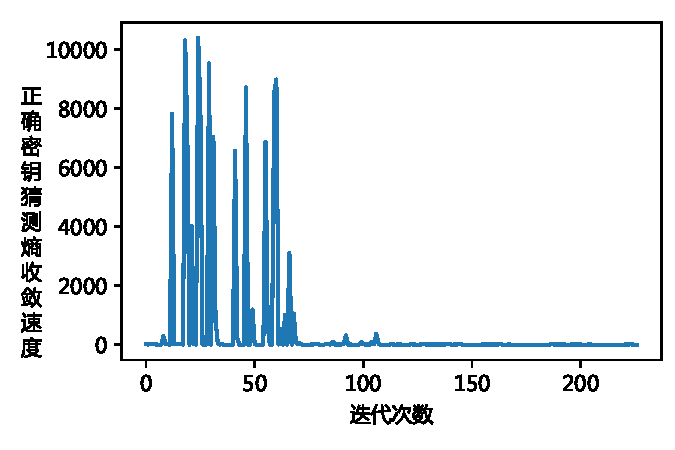
\includegraphics[width=\textwidth]{convratedpav4}
			\caption{DPA v4}
			\label{fig:convratedpav4}
		\end{subfigure}%
		~% add desired spacing
		\begin{subfigure}[b]{\trif\textwidth}
			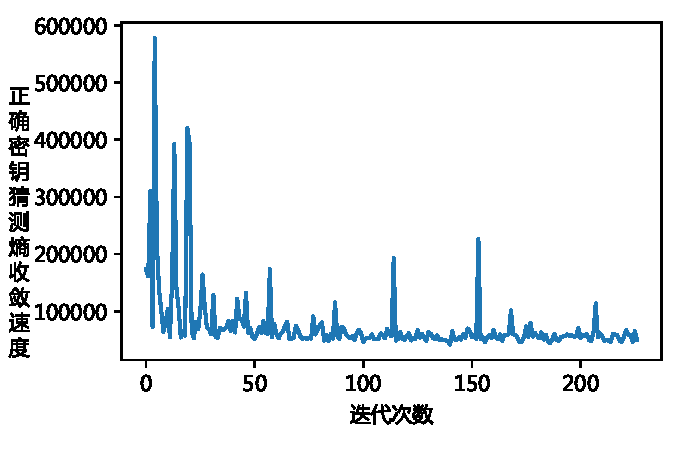
\includegraphics[width=\textwidth]{convrateaeshd}
			\caption{AES\_HD}
			\label{fig:convrateaeshd}
		\end{subfigure}
		~% add desired spacing
		\begin{subfigure}[b]{\trif\textwidth}
			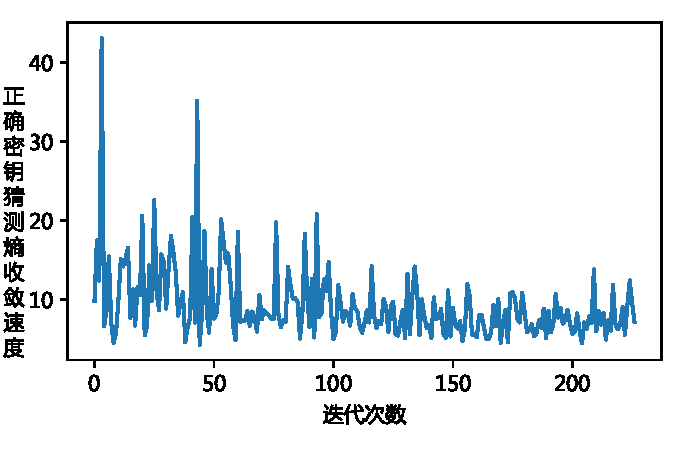
\includegraphics[width=\textwidth]{convrateaesrd}
			\caption{AES\_RD}
			\label{fig:convrateaesrd}
		\end{subfigure}
		\\% line break
		\begin{subfigure}[b]{\trif\textwidth}
			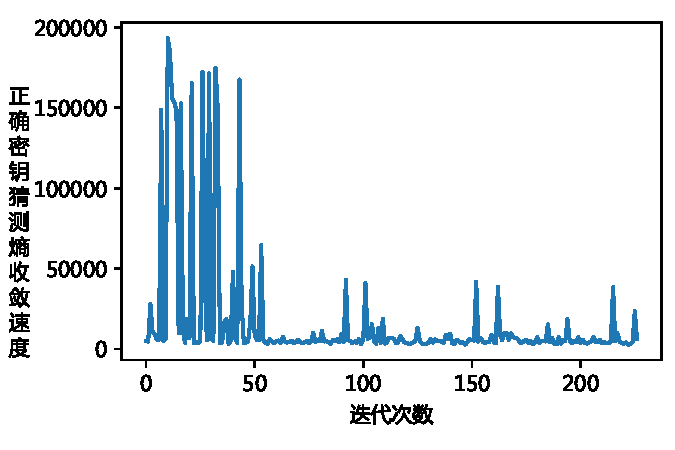
\includegraphics[width=\textwidth]{convrateascad0}
			\caption{ASCADf(N=0)}
			\label{fig:convrateascad0}
		\end{subfigure}%
		~% add desired spacing
		\begin{subfigure}[b]{\trif\textwidth}
			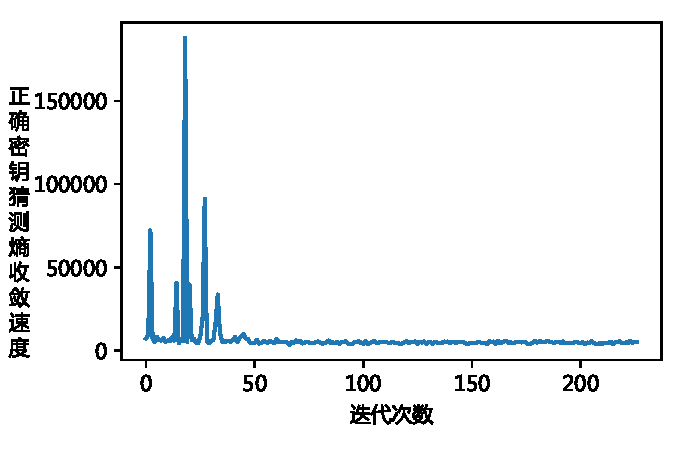
\includegraphics[width=\textwidth]{convrateascad50}
			\caption{ASCADf(N=50)}
			\label{fig:convrateascad50}
		\end{subfigure}
		~% add desired spacing
		\begin{subfigure}[b]{\trif\textwidth}
			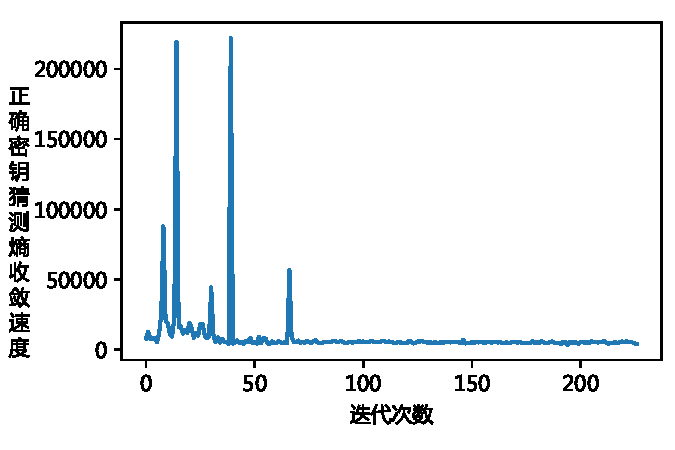
\includegraphics[width=\textwidth]{convrateascad100}
			\caption{ASCADf(N=100)}
			\label{fig:convrateascad100}
		\end{subfigure}
		\\% line break
		\bicaption{\enspace 深度学习训练过程的猜测上收敛速度曲线}{\enspace Curve of $convrate$ in Deep learning training process}
		\label{fig:convrateit}
	\end{figure}
	
	从\figureref{fig:convratedpav4},\figureref{fig:convrateaeshd},\figureref{fig:convrateascad0},\figureref{fig:convrateascad50}和\figureref{fig:convrateascad100}中可以看出,在搜索DPA v4、AES\_HD、ASCADf(N=0/N=50/N=100)数据集的最优数据增强策略参数时,在较早的阶段就达到较好的解并保持稳定,表明搜索快速收敛且找到了较优解。因此,在实际应用通用数据增强方法时可以减小迭代次数和提高退火速度以节省时间,并在攻击效果不受影响的前提下进行优化。\figureref{fig:convrateaesrd}展示了对AES\_RD数据集的搜索结果,攻击代价趋于稳定,在实际应用通用数据增强方法时可以不改变或略微增加迭代次数和降低退火速度来优化结果。
	
	可以看出,随着迭代次数的增加,代价逐渐降低并趋于稳定,这说明对于现有的数据集,将迭代次数设定为227可以使主控制器搜索出稳定的结果。
	
	本研究使用框架搜索到的所研究数据集的最佳数据增强策略参数如\tableref{tab:paras}所示。针对不同算法实现的能量迹,数据增强策略参数各异。参数的大致范围与理论一致,而其具体数值有必要使用本文通用数据增强方法进行搜索。
	
	\begin{table}[!h]
		\bicaption{\enspace 搜索到的最优数据增强策略参数}{\enspace Searched DA policy parameters}
		\label{tab:paras}
		\centering
		%\footnotesize% fontsize
		%\setlength{\tabcolsep}{4pt}% column separation
		%\renewcommand{\arraystretch}{1.2}%row space
		\small 
		\begin{tabular}{cc|cccccc}
			\hline
			\multicolumn{2}{c|}{\multirow{2}{*}{参数数值}} &\multirow{2}{*}{DPA v4}&\multirow{2}{*}{AES\_HD}&\multirow{2}{*}{AES\_RD}& \multicolumn{3}{c}{ASCAD} \\
			%\cline{3-5}
			\multicolumn{2}{c|}{}&&&&N=0 & N=50 & N=100 \\
			\hline
			\multirow{6}{*}{数据增强策略参数}
			&$p_{ro}$&0.676&0.720&0.762&0.161&0.749&0.621\\
			&$m_{ro}$&137&9&1&6&76&55\\
			&$p_{an}$&0.144&0.156&0.579&0.0761&0.444&0.774\\
			&$m_{an}$&   0&0.0523&0.345&0.522&0.0790&0.530\\
			&$p_{os}$&0.706&0.617&0.879&0.0579&0.0669&0.147\\
			&$m_{os}$&$10^{-5}$&0.399&0.0795&7.753&4.015&10\\
			\hline
			
		\end{tabular}   
	\end{table}

	\section{通用数据增强方法在AES算法实现分析中的实证研究}\label{sec:realexp}
	
	本文方法进行实证研究过程中,使用的机器配置如下:处理器型号为Intel(R) Xeon(R) CPU E5-2667 v4 @ 3.20GHz,内存大小252GB,操作系统版本为CentOS release 6.6 (Final)。本文方法使用Python(版本为3.6.2)作为编程语言进行实现,其中深度学习模型通过Keras\footnote{资料来源:keras \href{https://pypi.org/project/keras}{https://pypi.org/project/keras}。}开源框架进行实现。

	DL-SCA的攻击阶段与深度学习中的测试阶段有一定相似之处但并不完全相同。如\figureref{fig:dltestphase}和\figureref{fig:mydlscatest}所示,在深度学习训练出的模型对测试数据进行预测之后,还需要组合多条迹的信息进一步对算法密钥进行估计,从而计算侧信道领域的评价指标以评估侧信道分析技术效果,在本研究中,使用\chenggongtiaoshu 作为指标评估DL-SCA的效果,\chenggongtiaoshu 越小,那么DL-SCA效果越好。

	\begin{figure}[!h]
		\centering
		\begin{tikzpicture}[node distance=45pt, auto]
			% 定义节点样式
			\tikzstyle{reg} = [rectangle, draw,text centered]
			\tikzstyle{block} = [draw, rounded corners,align=center]
			\tikzstyle{data} = [draw, trapezium, trapezium left angle=70, trapezium right angle=110,align=center]
			\tikzstyle{arrow} = [thick,->,>=stealth]
			
			% 绘制节点
			\node [reg] (hyperparareg) {超参数寄存器};
			\node [block,below of =hyperparareg] (trained) {深度神经网络};
			\node [reg, left=70pt of trained] (parareg) {参数寄存器};
			\node [data, below of=trained] (dataset) {数据集};
			\node [block, right=100pt of dataset] (keypred) {密钥预测器};
			\node [block, below of =dataset] (keycalc) {密钥计算器};
			\node [block, below =50pt of keypred] (cmp) {侧信道分析\\指标计算器};
			
			%\node [block, below of=valacc, xshift=2cm] (testacc) {测试集准确率计算器};
			
			% 绘制箭头
			\draw [arrow] (dataset) -- node[right] {测试数据} (trained);
			\draw [arrow] (dataset) -- node[left] {测试标签(敏感中间值)} (keycalc);
			\draw [arrow] (dataset) -- node[pos=0.5,above] {算法输入、输出} (keypred);
			\draw [arrow] (dataset) -- ++(0:100pt) |- (keycalc);
			%\draw [arrow] (dataset) -- node[above] {测试数据} (pretrained);
			\draw [arrow] (trained) -| node[pos=0.3,above] {测试数据的标签预测结果} (keypred);
			\draw [arrow] (hyperparareg) -- node[right]{网络超参数}(trained);
			\draw [arrow] (parareg) -- node[above]{神经元参数}(trained);
			
			\draw [arrow] (keypred) -- node[right]{密钥预测值}(cmp);
			\draw [arrow] (keycalc) |- node[pos=0.7,below]{算法密钥}(cmp);
			\draw [arrow] (cmp) --node[pos=0.5, right] {\chenggongtiaoshu } ++(270:40pt);
		\end{tikzpicture}
		\bicaption{\enspace 攻击AES的深度学习测试阶段}{\enspace DL test phase for SCA on AES}
		\label{fig:mydlscatest}
	\end{figure}


	\subsection{通用数据增强方法的技术效果}
	
	本研究尝试了1倍、5倍、10倍、20倍四种增广倍数$C$(见\algorithmref{alg:combined-da}输入,$T^{agmt}=T*C$,$T$是数据增强前训练样本数量)以探索最优的实验条件。
	
	不同实验条件下DL-SCA的性能如\tableref{tab:adamtd}所示,表格中加粗的结果表示在对应数据集上取得的最优技术效果。根据实验结果可以看出,增广倍数为10倍或20倍时能取得最小的\chenggongtiaoshu 。例如,在分析引入随机延迟的软件AES实现数据集AES\_RD时,选取C=20。这样一来,在仅提供20000条能量迹用于DL-SCA的建模时,采用本文提出的数据增强方法可以将\chenggongtiaoshu 减小到5。在每个数据集上取得的最优技术效果的猜测熵曲线如\appfigureref{appfig:adadlsca}所示。
	
	\begin{table}[!h]
		\bicaption{\enspace 采用通用数据增强方法的DL-SCA的性能}{\enspace Performance of DL-SCA with general DA method}
		\label{tab:adamtd}
		\centering
		\footnotesize% fontsize
		%\setlength{\tabcolsep}{4pt}% column separation
		%\renewcommand{\arraystretch}{1.2}%row space
		\begin{tabular}{cc|cccccc}
			\hline
			\multirow{2}{*}{性能指标}&\multirow{2}{*}{增广倍数} &\multirow{2}{*}{DPA v4}&\multirow{2}{*}{AES\_HD}&\multirow{2}{*}{AES\_RD}& \multicolumn{3}{c}{ASCAD} \\
			%\cline{3-5}
			\multicolumn{2}{c|}{}&&&&N=0 & N=50 & N=100 \\
			\hline
			\multirow{2}{*}{\shortstack{数据增强前\\训练样本数量}}&&\multirow{2}{*}{4000}&\multirow{2}{*}{45000}&\multirow{2}{*}{20000}&\multirow{2}{*}{45000}&\multirow{2}{*}{45000}&\multirow{2}{*}{45000}\\
			&&&&&&&\\
			\hline
			\multirow{4}{*}{\chenggongtiaoshu }
			&1&9&1358&11&>300&>400&>400\\
			&5&4&959&6&>300&273&>400\\
			&10&\textbf{3}&\textbf{880}&6&\textbf{197}&305&\textbf{288}\\
			&20&\textbf{3}&898&\textbf{5}&206&\textbf{193}&382\\
			\hline
			
		\end{tabular}   
	\end{table}
	
%	使用本文提出的通用数据增强方法搜索最优的数据增强策略参数,使用这些参数对训练集进行组合式数据增强,使用数据增强后的训练集训练深度学习模型后,训练后的深度学习模型进行攻击的结果如\appfigureref{appfig:adadlsca}所示。我们从\appfigureref{appfig:adadlsca}提取\chenggongtiaoshu 的信息,将它们列举在\tableref{tab:adamtd}中。
%	
%	\begin{table}[!h]
%		\bicaption{\enspace 使用通用数据增强方法时DL-SCA的性能}{\enspace Performance of DL-SCA with adaptive DA method}
%		\label{tab:adamtd}
%		\centering
%		%\footnotesize% fontsize
%		%\setlength{\tabcolsep}{4pt}% column separation
%		%\renewcommand{\arraystretch}{1.2}%row space 
%		\begin{tabular}{c|cc}
%			\hline
%			数据集名称&数据增强前的训练样本数量&\chenggongtiaoshu \\
%			\hline
%			DPA v4    &4000&3\\
%			\hline
%			AES\_HD   &45000&860\\
%			\hline
%			\multirow{2}{*}{AES\_RD}
%				&5000&10\\
%				&20000&5\\
%			\hline
%			\multirow{2}{*}{ASCADf(N=0)}
%				&38400&255\\
%				&45000&197\\
%			\hline
%			ASCADf(N=50)&45000&156\\
%			\hline
%			ASCADf(N=100)&45000&288\\
%			\hline
%		\end{tabular}
%	\end{table}
	\subsection{无数据增强的技术效果}
	不进行数据增强,直接训练深度学习模型,并使用训练后的深度学习模型进行攻击的结果如\appfigureref{appfig:origindlsca}所示。我们从\appfigureref{appfig:origindlsca}提取\chenggongtiaoshu 的信息,将它们列举在\tableref{tab:originmtd}中。
	
	\begin{table}[!h]
		\bicaption{\enspace 无数据增强时DL-SCA的性能}{\enspace Performance of DL-SCA without any DA method}
		\label{tab:originmtd}
		\centering
		%\footnotesize% fontsize
		%\setlength{\tabcolsep}{4pt}% column separation
		%\renewcommand{\arraystretch}{1.2}%row space 
		\begin{tabular}{c|cc}
			\hline
			数据集名称&训练样本数量&\chenggongtiaoshu \\
			\hline
			DPA v4    &4000&4\\
			\hline
			AES\_HD   &45000&1118\\
			\hline
			\multirow{2}{*}{AES\_RD}
			&5000&12\\
			&20000&5\\
			\hline
			\multirow{2}{*}{ASCADf(N=0)}
			&38400&294\\
			&45000&259\\
			\hline
			ASCADf(N=50)&45000&369\\
			\hline
			ASCADf(N=100)&45000&304\\
			\hline
		\end{tabular}
	\end{table}

	对比\tableref{tab:adamtd}和\tableref{tab:originmtd}相对应(建模能量迹条数相同)的表项,可以观察到本文提出的方法在AES\_HD、DPA v4、ASCADf三种数据集共五个场景上使得\chenggongtiaoshu 减少21\%、25\%、24\%、48\%以及5\%。这说明与未采用数据增强的方法相比,采用本文提出的通用数据增强方法在无防护、高噪声、随机延迟或掩码防护的密码算法实现的DL-SCA场景中,能够显著提升侧信道分析技术效果,减少\chenggongtiaoshu 。上述结果表明,本文提出的数据增强方法的通用性。
	
	而在AES\_RD数据集上,\chenggongtiaoshu 保持不变,可能的原因是迭代次数不足。从\figureref{fig:convrateaesrd}中可以看出,AES\_RD数据集上攻击代价的在227的迭代次数下还未稳定;\figureref{fig:convratedpav4},\figureref{fig:convrateaeshd},\figureref{fig:convrateascad0},\figureref{fig:convrateascad50}和\figureref{fig:convrateascad100}中,其他数据集上攻击代价在227的迭代次数下已经达到稳定。出于公平比较的目的,我们限制了主控制器迭代次数为227。
	
%如果使用通用数据增强方法的DL-SCA的数据增强前的训练样本数量和无数据增强时DL-SCA的训练样本数量相同,那么前者的\chenggongtiaoshu 不高于后者的\chenggongtiaoshu 。例如,对于DPA v4数据集所对应的无防护软件实现,\tableref{tab:adamtd}的结果表明如果攻击者可以采集4000条迹进行建模,那么使用通用数据增强方法时,DL-SCA可以使用3条迹就完成攻击。同样对于DPA v4数据集所对应的无防护软件实现,\tableref{tab:originmtd}的结果表明如果攻击者可以采集4000条迹进行建模,那么不使用数据增强方法时,DL-SCA需要4条迹才能完成攻击。
%
%	通用数据增强相比于无数据增强,可以在攻击者采集相同数量的样本的情况下,使得深度学习模型对信息泄漏的刻画更准确,从而减少\chenggongtiaoshu 。本文提出的方法在AES\_HD、DPA v4、ASCADf(N=0)、ASCADf(N=50)、ASCADf(N=100)五个数据集上使得\chenggongtiaoshu 相比于无数据增强减少23\%、25\%、24\%、58\%以及5\%,在AES\_RD数据集上使得\chenggongtiaoshu 与无数据增强相当。
	\subsection{其他数据增强方法的技术效果}

	本文还将采用本文提出通用数据增强方法的DL-SCA和近年来采用其他数据增强方法的DL-SCA结果进行比较,以说明本文通用数据增强方法的优势。
	
	使用其他文献中的方法进行数据增强,最终进行DL-SCA的结果如\tableref{tab:othermtd}所示。
	
	%使用其他文献中的方法进行数据增强,最终进行DL-SCA的结果如\tableref{tab:othermtd}所示。在\tableref{tab:othermtd}中,“文献\normalcite{Cagli17}”表示本研究复现的\citet{Cagli17}位移变形和添加删除变形的数据增强方法,这是因为原文并无DPA v4、AES\_HD、AES\_RD和ASCADf数据集上的实验结果。“文献\normalcite{Kim19}”表示本研究复现的\citet{Kim19}添加高斯白噪声的数据增强方法,这是因为复现时使用的网络模型优于论文原本使用的网络模型,复现论文方法的实验结果优于论文所汇报的实验结果。“文献\normalcite{Won20}”表示\citet{Won20}使用合成少数类过采样法及其变体的数据增强方法,表项直接使用论文所汇报的实验结果。“文献\normalcite{Luo21}”表示\citet{Luo21}使用混淆技术的数据增强方法,表项直接使用论文所汇报的实验结果。“文献\normalcite{Mukhtar22}”表示\citet{Mukhtar22}基于条件生成对抗网络和连体网络的数据增强方法,表项直接使用论文所汇报的实验结果。

	\begin{table}[!h]
		\bicaption{\enspace 使用其他数据增强方法时DL-SCA的性能}{\enspace Performance of DL-SCA with other DA method}
		\label{tab:othermtd}
		\centering
		%\footnotesize% fontsize
		%\setlength{\tabcolsep}{4pt}% column separation
		%\renewcommand{\arraystretch}{1.2}%row space
		\footnotesize
		\begin{tabular}{cc|cccccc}
			\hline
			\multirow{2}{*}{数据增强方法} &\multirow{2}{*}{性能指标} &\multirow{2}{*}{DPA v4}&\multirow{2}{*}{AES\_HD}&\multirow{2}{*}{AES\_RD}& \multicolumn{3}{c}{ASCAD} \\
			%\cline{3-5}
			\multicolumn{2}{c|}{}&&&&N=0 & N=50 & N=100 \\
			\hline
			\multirow{2}{*}{Cagli等\citep{Cagli17}}
				&数据增强前训练样本数量       &4000&45000&20000&45000&45000&45000\\
				&\chenggongtiaoshu      &5&1252&7&219&328&364        \\
			\hline
			\multirow{2}{*}{Kim等\citep{Kim19}}
				&数据增强前训练集大小       &4000&45000&20000&45000&45000&45000\\
				&\chenggongtiaoshu     &5&1127&5&249&276&346\\
			\hline
			\multirow{2}{*}{Won等\citep{Won20}}
				&数据增强前训练集大小       &/&/&5000&/&/&45000\\
				&\chenggongtiaoshu     &/&/&15&/&/&190\\
			\hline
			\multirow{2}{*}{Luo等\citep{Luo21}}
				&数据增强前训练集大小       &/&/&50000&50000&50000&50000\\
				&\chenggongtiaoshu     &/&/&>1000&1250&4000&7000\\
			\hline
			\multirow{2}{*}{Mukhtar等\citep{Mukhtar22}}
				&数据增强前训练集大小       &/&/&/&38400&/&/\\
				&\chenggongtiaoshu     &/&/&/&410&/&/\\
			\hline
			
		\end{tabular}   
	\end{table}

	对比\tableref{tab:adamtd}、\tableref{tab:originmtd}和\tableref{tab:othermtd}相对应(建模能量迹条数相同)的表项,可以观察到在AES\_RD、AES\_HD、DPA v4、ASCADf(N=0/N=50)四种数据集五个场景中,采用本文方法的DL-SCA\chenggongtiaoshu 减小比例最高。与已有最好的数据增强方法相比,采用本文提出的数据增强方法可将实施侧信道分析的\chenggongtiaoshu 分别降低0\%、22\%、40\%、10\%、30\%。这说明,与采用了数据增强的已知最好方法相比,采用本文提出的通用数据增强方法,在无防护、高噪声或掩码防护型密码算法实现的DL-SCA场景中,本文提出的数据增强方法更高效。

	在ASCADf(N=100)数据集上,与最好的数据增强方法Won等\citep{Won20}相比,采用本文提出的数据增强方法使得实施侧信道分析的\chenggongtiaoshu 增加52\%。可能的原因是Won等\citep{Won20}尝试85种SMOTE算法的不同变体找到一种较优的数据增强方法,而本文方法仅对三种数据增强子策略进行组合式数据增强并搜索最优参数。因此在实际应用中,本文方法更容易满足时间效率的需求,可以高效地找到合适的数据增强策略参数。除此之外,增加数据增强子策略到通用数据增强方法的数据增强单元,有可能使得本文方法达到与Won等\citep{Won20}匹配的结果。
	%通用数据增强相比于无数据增强,可以在攻击者采集相同数量的样本的情况下,有较大的可能使得深度学习模型对信息泄漏的刻画更准确,从而减少\chenggongtiaoshu 。本文提出的方法在AES\_HD、DPA v4、ASCADf(N=0)、ASCADf(N=50)四个数据集上使得\chenggongtiaoshu 相比于已知最好的数据增强方法分别减少24\%、40\%、10\%、43\%,在AES\_RD数据集上使得\chenggongtiaoshu 与已知最好的数据增强方法相当,在ASCADf(N=100)数据集上使得\chenggongtiaoshu 相比于已知最好的数据增强方法增加了52\%。
	\section{本章小结}
	针对已有数据增强方法的参数选取高度依赖专家知识,且只适用于特定算法实现数据集的实际问题,本文提出一种通用数据增强方法,该方法能够自适应地搜索数据增强策略参数,增广出新的样本用于训练深度学习模型,进而提升DL-SCA效果。本文通过对应于多种攻击难度的AES算法实现的数据集对新提出的通用数据增强方法进行了验证。实验结果表明,与无数据增强或目前已知的数据增强方法相比,通用数据增强方法可以使得\chenggongtiaoshu 最多降低48\%。
}